% =============================================================================
% Project : THE_PHILOSOPHY_OF_VIABILITY
% Book    : Book I — Ontology of Viability
% Book ID : VS.B01
%
% File    : 2_MAINMATTER/PART_I_IDENTITY_AND_MANIFESTATION/CHAPTER_03_UNITY_AND_PLURALITY/sections/section_08_limits_of_unity_and_plurality.tex
%
% Section:
%   Section 08 — Limits of Unity and Plurality
%
% Purpose :
%   To establish the ontological and inferential limits of claims
%   concerning unity and plurality; distinguish what can be
%   established about a subject from what remains unresolved
%   concerning identity, source, aggregate, composition,
%   manifestation, and ontological respect; and prevent the
%   unrestricted transfer of conclusions from one determination
%   to another.
%
% Conceptual Policy:
%   1. Neither unity nor plurality is treated as a universal
%      ontological priority.
%   2. Every claim must specify its subject, respect, domain,
%      and scope.
%   3. Multiplicity does not automatically establish plurality
%      of identities.
%   4. Unity does not automatically establish singular identity.
%   5. Source, aggregate, composition, structure, manifestation,
%      and identity remain distinct ontological questions.
%   6. Numerical classification does not determine identity-number.
%   7. Conclusions must not exceed the grounds that support them.
%   8. Unresolved questions remain explicitly open.
%
% =============================================================================

\section{Limits of Unity and Plurality}
\label{sec:limits-of-unity-and-plurality}

% -----------------------------------------------------------------------------
\subsection{The Need to Establish the Limits of Unity and Plurality}

The preceding sections have examined unity and plurality
through several distinct ontological questions. They have
distinguished unity of identity from unity of source,
aggregate, and composition; examined the possibility of
plurality within a configuration; differentiated multiplicity
from plurality of identities; and rejected the equivalence
of unity with numerical singularity. These distinctions
establish a necessary conceptual basis, but they do not
by themselves determine the full scope of either unity
or plurality.

A further problem must therefore be addressed: what may
legitimately be inferred when unity or plurality has been
established, and where must the inference stop? An
ontological determination may be valid within a specified
respect without being valid in every other respect. A
claim may accurately describe the organization of a
composition while leaving the identity of that composition
unresolved. Likewise, a plurality of manifestations may
be established without determining whether the identities
involved are one or multiple.

Without explicit limits, unity and plurality can become
unrestricted explanatory principles. Unity may be invoked
to explain every form of coherence, organization, relation,
or identity, while plurality may be invoked to explain
every form of distinction, differentiation, or internal
multiplicity. Both uses exceed what these determinations
can establish on their own. The task of this section is
therefore not to diminish the ontological significance
of unity or plurality, but to delimit the conclusions
that can be drawn from them.

The limits considered here are not merely limitations
of language or classification. They concern the validity
of ontological inference. A determination established
in one respect cannot be transferred to another simply
because the same existent is involved in both claims.
The subject may remain the same while the ontological
question changes. The analysis must therefore distinguish
the subject under examination from the particular
determination attributed to it.

% -----------------------------------------------------------------------------
\subsection{The Limit of Unity as a Universal Principle}

Unity cannot be assumed to be the universal ontological
ground of every existent or every determination of an
existent. The recognition that a subject is unified in
a particular respect does not establish that all of its
determinations, components, relations, and manifestations
derive from one undifferentiated unity. Nor does it
establish that every entity related to that subject
belongs to one identity or is absorbed into one ontological
whole.

The unity attributed to a source, for example, does not
automatically determine the identity of everything related
to that source. A common source may be relevant to the
origin, constitution, or relation of several entities,
but the identity relations among those entities remain
a separate question. Similarly, the unity of an aggregate
does not establish that its components constitute one
identity. The unity of a composition may concern its
organization without settling the identity status of
the composed subject or the components involved.

A universal principle of unity would also risk treating
every plurality as merely apparent or derivative. Such
a conclusion cannot be obtained from the recognition
of unity in a particular subject. If several entities
are related within a unified configuration, their
distinctions cannot be eliminated merely by referring
to the unity of that configuration. The relation between
the unity of the broader subject and the distinctions
among its constituents requires independent examination.

Unity may therefore be ontologically significant without
being an exhaustive explanation of every relation within
or beyond its subject. Its explanatory scope must remain
limited to the respect in which it has been established.
Any extension beyond that respect requires additional
grounds identifying the relevant relation and explaining
why the original unity claim applies to the further
subject or determination.

% -----------------------------------------------------------------------------
\subsection{The Limit of Plurality as a Universal Principle}

Plurality cannot be assumed to be the universal
ontological condition of every existent. The presence
of multiple determinations, components, relations,
manifestations, or processes does not establish that
the subject consists of multiple identities. These
forms of multiplicity may be ontologically relevant,
but their relevance does not make them interchangeable
with identity plurality.

A plurality of components may belong to a composition
whose identity remains a separate question. Multiple
relations may determine or connect a subject without
each relation constituting an identity. Several
manifestations may be associated with an existent
without their number determining the number of
identities involved. In each case, the plurality
established concerns a specified kind of element,
not automatically the identity of the broader subject.

The universalization of plurality would produce an
opposite reduction to the universalization of unity.
It would treat every internal difference as evidence
of multiple identities and every differentiated
configuration as ontologically plural in the same
respect. That inference would confuse the existence
of distinctions with the ontological status of the
distinguished items. Distinction is relevant to an
analysis of plurality, but the kind and significance
of the distinction must still be established.

Plurality is therefore indispensable where multiple
subjects or elements are established within a specified
domain and respect. It cannot replace the analysis
of what is being distinguished, what kind of plurality
is involved, and whether that plurality has any
implication for identity. The transition from a
plurality of elements to a plurality of identities
requires an independent ontological argument.

% -----------------------------------------------------------------------------
\subsection{The Limit of Inferring Identity from Unity}

Unity alone cannot determine the number or structure
of identities. An existent may be described as unified
as an aggregate, a composition, a material configuration,
a relational arrangement, or a structured whole. Such
descriptions may establish unity within particular
respects, but they do not independently establish
that exactly one identity is involved.

The following inference is therefore insufficient:

\[
\text{Unity of a Subject}
\not\Rightarrow
\text{Exactly One Identity}.
\]

The insufficiency does not arise because unity is
irrelevant to identity. Unity may be relevant to an
identity-related investigation, and in some cases
a unity claim may form part of an argument concerning
identity. The problem is that the unity claim alone
does not supply the additional premises required to
determine identity-number. The subject of unity may
not be identical with the subject whose identity
is being investigated, and the respect in which
unity is established may not be the respect relevant
to identity.

To infer singular identity from unity, an account
would have to establish at least the relevant identity
subject, the grounds on which its identity is determined,
and the relation between those grounds and the unity
already established. It would also have to exclude
the possibility that the unity belongs to an aggregate,
composition, or configuration involving more than
one identity. Without such an account, the conclusion
exceeds the premises.

This restriction does not deny the possibility of
singular identity. It prevents singular identity
from being treated as an automatic consequence of
unity. The conclusion may be established in a
particular case, but it must be supported by an
argument appropriate to identity rather than inferred
from the use of the term ``one'' or from a unity
attributed to another ontological subject.

% -----------------------------------------------------------------------------
\subsection{The Limit of Inferring Identity from Plurality}

Plurality alone cannot determine the number of
identities either. The presence of several components,
relations, determinations, manifestations, or processes
does not establish that each constitutes a distinct
identity. The inference from plurality to identity
multiplicity therefore exceeds what the recognition
of plurality alone can support.

This restriction may be expressed as:

\[
\text{Plurality of Elements}
\not\Rightarrow
\text{Plurality of Identities}.
\]

The expression ``plurality of elements'' must itself
be specified. Components may be materially distinct,
relations may be numerically multiple, manifestations
may differ in form, and determinations may be
distinguishable under different respects. These
pluralities do not necessarily have the same
ontological status. Even when each plurality is
correctly established, the identity question remains:
what is the relation between the distinguished
elements and the identity or identities under
consideration?

A plurality of components may belong to one
composition, but this possibility does not establish
that every composition has one identity. Several
manifestations may be related to one existent, but
this possibility does not establish that all
manifestations in every case belong to one identity.
Multiple relations may participate in the determination
of a subject without independently establishing
multiple identities. Each example limits an inference;
none supplies a universal conclusion about identity-number.

The converse reduction must also be avoided. The
failure of plurality of elements to prove plurality
of identities does not prove that only one identity
is involved. The absence of a sufficient argument
for plurality is not a sufficient argument for unity.
The identity status of the subject must remain open
where the relevant ontological grounds have not
been established.

% -----------------------------------------------------------------------------
\subsection{The Limits of Source-Based Explanations}

The distinction between source and aggregate places
an important restriction on explanations of unity
and plurality. A source may be relevant to the
constitution, origin, or relation of multiple entities
or manifestations. However, the existence of a common
source does not automatically establish that all
related entities possess one identity. A source
relation is not, merely by being common, an identity
relation.

The plurality of manifestations also cannot be used
to infer the plurality of sources without an
independent argument. Several manifestations may
be related to one source, while a plurality of
sources may also be related to a broader configuration.
The number of manifestations and the number of
sources are distinct questions. Neither can be
determined solely by counting the other.

A source-based explanation must therefore specify
what is meant by source and what relation is being
asserted. It must distinguish origin, production,
dependence, constitution, and association wherever
these relations are relevant. These relations may
have different ontological implications. A common
origin does not necessarily imply present identity;
a relation of dependence does not necessarily imply
composition; and a shared source does not necessarily
establish a single identity among the entities
related to it.

The same restriction applies to the unity of source.
Even if a source is established as one in a particular
respect, the unity of that source cannot simply be
transferred to its manifestations or effects. The
ontological status of what is related to a source
must be examined in its own right. Source may explain
a relation, but it cannot substitute for an account
of identity.

% -----------------------------------------------------------------------------
\subsection{The Limits of Aggregate and Compositional Unity}

An aggregate may possess unity as an organized,
bounded, or related configuration. A composition
may also exhibit unity through the organization
or interrelation of its components. Such unity
may be significant for understanding the subject,
but it does not automatically establish that the
aggregate or composition constitutes one identity.

The components of an aggregate or composition may
retain distinctions that cannot be eliminated
merely by describing them as parts of one whole.
Their material, structural, relational, or other
determinations may remain relevant to their
ontological status. Conversely, the presence of
multiple components does not establish that the
aggregate lacks every form of unity. The plurality
of components and the unity of the composed
configuration may concern different respects.

The following restrictions must therefore be
maintained:

\[
\text{Unity of Composition}
\not\Rightarrow
\text{Unity of Identity}
\]

\[
\text{Plurality of Components}
\not\Rightarrow
\text{Plurality of Identities}.
\]

These restrictions prevent composition from becoming
either a universal foundation of identity or an
automatic negation of unity. They also prevent
the number of components from being treated as
a direct measure of the number of identities.

The philosophical debate concerning material
composition illustrates why the relation between
parts and wholes cannot be assumed to have one
uncontroversial solution. Different accounts
disagree about when parts compose an object and
what ontological status should be assigned to
ordinary composite entities. These debates are
relevant as comparative problems, but no particular
solution to the problem of composition is adopted
here as a premise for the ontology of identity.\footnote{For contrasting approaches to material composition and the relation between parts and wholes, see Peter van Inwagen, \textit{Material Beings} (1990), and Peter Simons, \textit{Parts: A Study in Ontology} (1987), both recorded in the bibliography of this volume.}

The ontological status of an aggregate or composition
must therefore be examined through more than the
number or arrangement of its components. Its unity,
if established, must be specified; the identity
or identities involved must be independently
examined; and no conclusion about one of these
questions should be transferred to the others
without justification.

% -----------------------------------------------------------------------------
\subsection{The Limits of Manifestational Inference}

Plurality of manifestations introduces a further
limit. An existent may exhibit several manifestations
without this plurality necessarily establishing
multiple identities. Different manifestations may
be related to one identity, to more than one identity,
or to an identity relation that cannot be determined
from manifestation alone. The plurality of
manifestations does not settle these alternatives.

The opposite assumption is equally unjustified.
Different manifestations must not automatically
be treated as merely different appearances of one
identity. Such a claim would already presuppose
the unity of identity that the analysis is meant
to examine. The relation between an existent and
its manifestations must be investigated without
assuming in advance either identity unity or
identity plurality.

Manifestational difference may be relevant to an
identity-related inquiry. It may indicate that
different determinations, modes of appearance,
or relational conditions are involved. But relevance
is not sufficiency. The existence of a difference
among manifestations does not by itself establish
a difference among identities, just as the
continuity or relatedness of manifestations does
not by itself establish one identity.

% =============================================================================
% Project : THE_PHILOSOPHY_OF_VIABILITY
% Book    : Book I — Ontology of Viability
% Book ID : VS.B01
%
% File    : 4_ASSETS/illustrations/VS.B01.P01.C03.S08.SS08.P003.IL01.manifestation_plurality_and_identity_scope.tex
%
% Asset:
%   Illustration IL01 — Manifestation Plurality and Identity Scope
%
% Purpose :
%   To illustrate that multiple manifestations can be distinguished
%   without deciding, solely on that basis, whether one or multiple
%   identities are involved.
%
% =============================================================================

\begin{figure}[htbp]
\centering

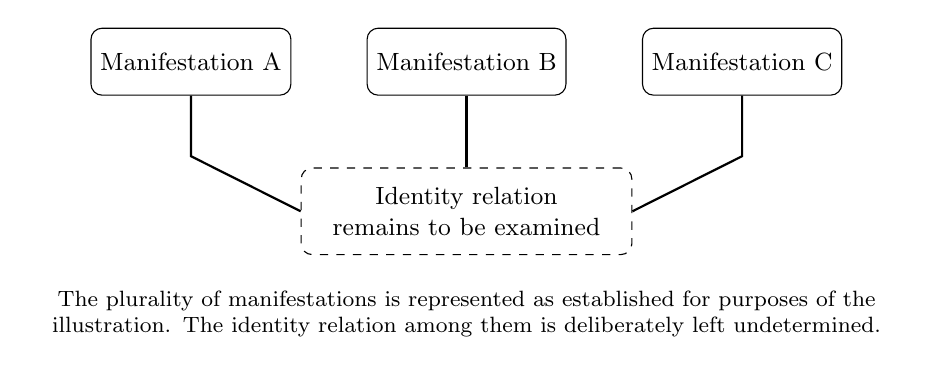
\begin{tikzpicture}[
    manifestation/.style={
        draw,
        rounded corners,
        minimum width=2.1cm,
        minimum height=0.85cm,
        align=center,
        font=\small
    },
    question/.style={
        draw,
        rounded corners,
        dashed,
        minimum width=4.2cm,
        minimum height=1.1cm,
        align=center,
        font=\small
    },
    relation/.style={
        thick,
        -
    }
]

\node[manifestation] (m1) at (-3.5,1.5) {Manifestation A};
\node[manifestation] (m2) at (0,1.5) {Manifestation B};
\node[manifestation] (m3) at (3.5,1.5) {Manifestation C};

\node[question] (identity) at (0,-0.4) {
    Identity relation\\
    remains to be examined
};

\draw[relation] (m1.south) -- (-3.5,0.3) -- (identity.west);
\draw[relation] (m2.south) -- (identity.north);
\draw[relation] (m3.south) -- (3.5,0.3) -- (identity.east);

\node[
    align=center,
    text width=0.9\textwidth,
    font=\footnotesize
] at (0,-1.7) {
    The plurality of manifestations is represented as established
    for purposes of the illustration. The identity relation among
    them is deliberately left undetermined.
};

\end{tikzpicture}

\caption{Plurality of Manifestations and the Unresolved Identity Relation}
\label{fig:manifestation-plurality-and-identity-scope}
\end{figure}

% =============================================================================
% END OF ILLUSTRATION IL01
% =============================================================================

The illustration distinguishes the plurality of
manifestations from the identity question associated
with them. It deliberately leaves the identity
relation unresolved: the diagrammatic grouping of
manifestations is not intended to assert that
they necessarily belong to one identity or to
multiple identities. Its purpose is to make visible
the gap between a manifestational description
and an identity conclusion.

The relation between manifestation and identity
therefore remains an independent ontological problem.
Any conclusion concerning identity must be supported
by grounds that address the identity relation itself,
rather than by the number, similarity, difference,
or grouping of manifestations alone.

% -----------------------------------------------------------------------------
\subsection{The Limit of Numerical Enumeration}

Numerical enumeration cannot provide an exhaustive
account of unity or plurality. Counting requires
a domain of enumeration, a criterion of distinction,
and a specification of what is being counted.
Different criteria may produce different numerical
descriptions of the same broader configuration.
A composition may be counted as one composed
subject while its components are counted as several
elements. A broader configuration may be counted
as one aggregate while several existents remain
distinguishable within it.

Such descriptions are not necessarily contradictory
because they may concern different subjects or
respects. Their compatibility, however, does not
mean that numerical classification is arbitrary.
A count may be precise within its intended domain.
Its limitation concerns the range of conclusions
that may legitimately be drawn from it.

Numerical variation does not by itself determine
the ontological number of identities. The criterion
of enumeration may identify components, material
units, relations, manifestations, or aggregates,
but the identity status of the counted items
requires a separate analysis. A count of several
components is not yet a count of several identities;
a count of one aggregate is not yet a count of
one identity.

The distinction is particularly important when
a numerical description is transferred from one
level of analysis to another. The fact that a
configuration is one under a criterion of
aggregation does not establish that it is one
under a criterion relevant to identity. Likewise,
the fact that several units are distinguished
under a material or relational criterion does
not establish that several identities are involved.

Numerical classification may therefore contribute
to ontological analysis, but it cannot replace it.
The ontological significance of a numerical result
must be established through an account of the
relation between the counted subject, the criterion
of enumeration, and the determination under
investigation.

% -----------------------------------------------------------------------------
\subsection{The Limit of Treating Unity and Plurality as Opposites}

Unity and plurality are often presented as
mutually exclusive alternatives. This opposition
becomes misleading when the relevant subject,
domain, and ontological respect are not specified.
A configuration may be unified in one respect
and plural in another. The unity of an aggregate
may coexist with the plurality of its components;
the unity of a source may coexist with the
plurality of its manifestations; and a broader
configuration involving multiple identities
may exhibit unity under a different determination.

These possibilities do not establish that every
form of unity and plurality can coexist without
qualification. If unity and plurality are attributed
to the same subject, in the same respect, under
the same conditions, their compatibility cannot
simply be assumed. The apparent opposition must
be examined to determine whether the claims
actually concern the same determination or whether
one of them changes its subject, scope, or criterion.

The distinction between respects is therefore
not a device for dissolving every contradiction.
It is a requirement for identifying the content
of each claim. If the subjects or respects differ,
the claims may be compatible. If they are identical,
a further account is required to determine whether
the predicates are genuinely incompatible or
whether the terms have been used in different senses.

Unity and plurality must consequently not be
treated as unrestricted logical opposites. Their
relation depends on what is unified, what is plural,
and the respect in which each determination is
asserted. A conclusion about compatibility or
incompatibility must follow from that analysis,
not from the words alone.

% -----------------------------------------------------------------------------
\subsection{The Limits of Reduction to One Ontological Respect}

Unity and plurality cannot be adequately examined
when all ontological determinations are reduced
to a single respect. Material constitution,
composition, structural organization, relational
determination, manifestation, and identity are
not interchangeable categories. They may be
related within an existent, but the relation
does not make their respective questions identical.

A plurality established in one of these respects
cannot automatically be transferred to another.
Material plurality does not necessarily establish
plurality of identity. Relational plurality does
not necessarily establish multiple existents.
Plurality of determinations does not necessarily
establish plurality of identities. Conversely,
unity in material constitution does not
automatically establish unity of identity, and
structural organization does not independently
prove that the organized subject has one identity.

Every inference across ontological respects
requires an account of the relation that makes
the inference legitimate. It is not enough to
point out that two determinations belong to
the same existent or configuration. Their
co-occurrence does not establish that one
determines the other. A relation of constitution,
dependence, realization, or manifestation may
be relevant, but its ontological significance
must be established rather than assumed.

The following diagram distinguishes several
respects in which unity or plurality may be
examined. It does not arrange them into a
hierarchy, nor does it assert that one respect
grounds or determines another.

% =============================================================================
% Project : THE_PHILOSOPHY_OF_VIABILITY
% Book    : Book I — Ontology of Viability
% Book ID : VS.B01
%
% File    : 4_ASSETS/diagrams/VS.B01.P01.C03.S08.SS12.P003.DG01.limits_of_inference_across_ontological_respects.tex
%
% Asset:
%   Diagram DG01 — Limits of Inference Across Ontological Respects
%
% Purpose :
%   To distinguish several ontological respects in which unity
%   and plurality may be examined, and to show that conclusions
%   established in one respect do not automatically transfer
%   to another.
%
% =============================================================================

\begin{figure}[htbp]
\centering

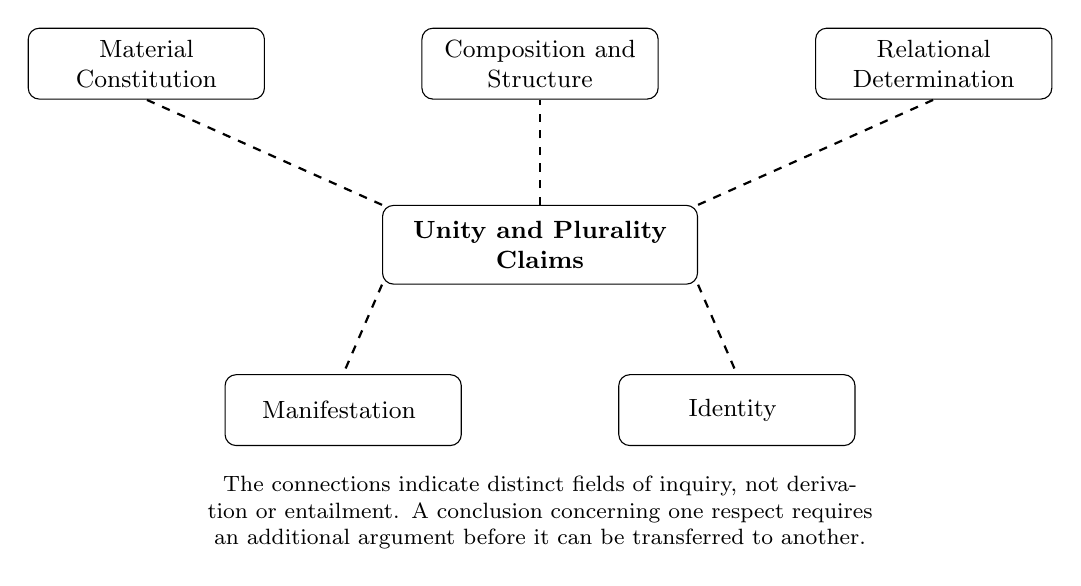
\begin{tikzpicture}[
    respect/.style={
        draw,
        rounded corners,
        align=center,
        minimum width=3.0cm,
        minimum height=0.9cm,
        font=\small
    },
    central/.style={
        draw,
        rounded corners,
        align=center,
        minimum width=4.0cm,
        minimum height=1.0cm,
        font=\small\bfseries
    },
    nonentailment/.style={
        dashed,
        thick,
        -
    }
]

\node[central] (inquiry) at (0,0) {
    Unity and Plurality\\
    Claims
};

\node[respect] (material) at (-5,2.3) {
    Material\\
    Constitution
};

\node[respect] (composition) at (0,2.3) {
    Composition and\\
    Structure
};

\node[respect] (relation) at (5,2.3) {
    Relational\\
    Determination
};

\node[respect] (manifestation) at (-2.5,-2.1) {
    Manifestation
};

\node[respect] (identity) at (2.5,-2.1) {
    Identity
};

\draw[nonentailment] (inquiry.north west) -- (material.south);
\draw[nonentailment] (inquiry.north) -- (composition.south);
\draw[nonentailment] (inquiry.north east) -- (relation.south);
\draw[nonentailment] (inquiry.south west) -- (manifestation.north);
\draw[nonentailment] (inquiry.south east) -- (identity.north);

\node[
    align=center,
    text width=0.92\textwidth,
    font=\footnotesize
] at (0,-3.4) {
    The connections indicate distinct fields of inquiry,
    not derivation or entailment. A conclusion concerning
    one respect requires an additional argument before
    it can be transferred to another.
};

\end{tikzpicture}

\caption{Limits of Inference Across Ontological Respects}
\label{fig:limits-of-inference-across-ontological-respects}
\end{figure}

% =============================================================================
% END OF DIAGRAM DG01
% =============================================================================

The diagram is an analytical map of possible
questions, not a complete inventory of the
ontology and not a causal or derivational model.
Its purpose is to prevent a determination
established in one respect from being transferred
to another without an explicit argument.

The reduction of all these questions to one
respect would conceal rather than resolve the
ontological problems under examination. A
satisfactory account must preserve the distinctions
while examining the relations among them.

% -----------------------------------------------------------------------------
\subsection{Unresolved Questions Concerning Identity and Number}

The restrictions established above leave several
ontological questions open. These questions are
not open merely because the relevant terms have
not yet been defined. They concern relations and
conditions that cannot be settled through unity,
plurality, or numerical classification alone.

Among the unresolved questions are:

\begin{itemize}
    \item Under what ontological conditions can
    an existent be established as involving
    exactly one identity?

    \item Under what conditions, if any, can
    multiple identities be involved in one
    existent or broader configuration?

    \item What grounds distinguish a plurality
    of manifestations from a plurality of identities?

    \item How are the identity boundaries of
    components related to the boundaries of
    a composition or aggregate?

    \item Can unity be established across
    different ontological respects without
    presupposing a single identity?

    \item What ontological relations connect
    a source with multiple manifestations
    without reducing source to manifestation
    or identity to source?

    \item What conditions make a distinction
    among elements relevant to identity rather
    than merely to material, structural,
    relational, or manifestational description?

    \item How should the possibility of identity
    plurality be assessed without presupposing
    that every existent has exactly one identity
    or that every differentiated configuration
    contains several identities?
\end{itemize}

These questions require further ontological
examination of identity, determination,
composition, relation, and manifestation.
They cannot be settled merely by defining
unity as oneness or plurality as multiplicity.
Nor should their openness be mistaken for
evidence that every proposed possibility
is equally established.

The present inquiry establishes restrictions
on what may be inferred. It does not claim
that the unresolved alternatives have already
been demonstrated. Their status must remain
provisional or open until the relevant
ontological grounds have been examined.

% -----------------------------------------------------------------------------
\subsection{Methodological Restrictions}

The analysis of unity and plurality must observe
a set of methodological restrictions. These
restrictions govern the formulation and evaluation
of ontological claims; they are not a substitute
for the substantive arguments required in each
particular case.

First, every claim of unity or plurality must
identify its subject. A statement that something
is one or multiple is incomplete if it does not
make clear what is being counted, unified,
distinguished, or related.

Second, the ontological respect and domain of
the claim must be specified. A conclusion
established concerning material constitution
cannot be transferred automatically to identity,
and a conclusion concerning manifestation
cannot be transferred automatically to source.

Third, numerical descriptions must not be treated
as complete ontological determinations. Counting
may be accurate within a domain while leaving
the identity status of the counted subject
unresolved.

Fourth, plurality of components, relations,
determinations, processes, or manifestations
must not be converted automatically into
plurality of identities. The ontological status
of the distinguished elements requires
independent examination.

Fifth, unity of source, aggregate, composition,
or structure must not be converted automatically
into unity of identity. Each form of unity
concerns a particular subject and respect.

Sixth, the distinction between unity and plurality
must not be used to impose a universal ontological
priority. Neither determination has been shown
to be an unrestricted ground from which all
other determinations can be derived.

Seventh, a distinction among respects must not
be introduced merely to protect a preferred
conclusion from criticism. The relevant respects
and their relations must be independently
specified, and apparent contradictions must
be examined rather than dismissed.

The methodological requirements and the
conclusions they restrict are summarized in
Table~\ref{tab:methodological-limits-of-unity-and-plurality}.

% =============================================================================
% Project : THE_PHILOSOPHY_OF_VIABILITY
% Book    : Book I — Ontology of Viability
% Book ID : VS.B01
%
% File    : 4_ASSETS/tables/VS.B01.P01.C03.S08.SS13.P003.TL01.methodological_limits_of_unity_and_plurality.tex
%
% Asset:
%   Table TL01 — Methodological Limits of Unity and Plurality
%
% Purpose :
%   To summarize the principal restrictions governing claims
%   about unity, plurality, and their implications for identity.
%
% =============================================================================

\begin{table}[htbp]
\centering
\caption{Methodological Limits of Unity and Plurality}
\label{tab:methodological-limits-of-unity-and-plurality}
\footnotesize
\renewcommand{\arraystretch}{1.2}

\begin{tabularx}{\textwidth}{
    @{}
    p{0.24\textwidth}
    X
    p{0.32\textwidth}
    @{}
}
\toprule
\textbf{Analytical Requirement} &
\textbf{Restriction} &
\textbf{Inference Not Licensed by Itself}
\\
\midrule

Specify the subject &
Identify what is unified, plural, counted, or distinguished. &
Unity of one subject establishes unity of another subject.
\\

Specify the respect &
Identify the ontological determination under examination. &
Material, relational, or manifestational plurality establishes identity plurality.
\\

Specify the domain &
Identify the range within which the claim is valid. &
A local numerical result applies to every ontological domain.
\\

Specify the criterion &
Identify what counts as one or multiple. &
Numerical classification determines ontological identity-number.
\\

Preserve conceptual distinctions &
Keep source, aggregate, composition, structure, manifestation, and identity distinct. &
Unity or plurality in one category settles another category.
\\

Establish cross-respect relations &
Provide grounds for transferring a conclusion between respects. &
Co-occurrence of determinations establishes entailment.
\\

Preserve unresolved questions &
Do not convert insufficient evidence into a universal conclusion. &
Failure to prove plurality establishes singular identity, or vice versa.
\\

\bottomrule
\end{tabularx}
\end{table}

% =============================================================================
% END OF TABLE TL01
% =============================================================================

These requirements define conditions for
responsible ontological inference. They do
not constitute a universal definition of
unity, plurality, or identity. Nor do they
settle the final structure of every existent.
Their function is to ensure that an argument
does not claim more than its premises and
ontological grounds establish.

% -----------------------------------------------------------------------------
\subsection{Conclusion: The Scope and Limits of Unity and Plurality}

Unity and plurality are indispensable for
examining the ontological organization of
existents. Their significance, however,
does not make either an unrestricted
explanation of identity, source, composition,
aggregate, structure, or manifestation.

Unity does not establish numerical singularity
or exactly one identity. Plurality does not
establish multiple identities. The unity
of a source or aggregate does not automatically
determine the identity of what is related
to it, and the plurality of components or
manifestations does not automatically
determine the plurality of identities involved.

The analysis has also established that
conclusions must remain within the scope
of the subject and respect for which they
were justified. A determination established
in one ontological respect may be relevant
to another, but relevance does not establish
entailment. The relation must be demonstrated
through an argument appropriate to the
ontological questions involved.

The unresolved questions concerning
identity-number and the relations among
identities must therefore remain open
where the available grounds do not settle
them. This openness is not an endorsement
of every possible answer. It is a refusal
to treat an unsupported inference as an
established ontological result.

The chapter's final section will synthesize
the distinctions developed throughout
the inquiry. It will identify the results
that can be retained, the claims whose
scope has been restricted, and the questions
that remain unresolved, without converting
those results into a premature universal
theory of unity, plurality, or identity.

% =============================================================================
% END OF SECTION 08 OF CHAPTER 03
% =============================================================================